\part{立体几何与线性代数初步}



\chapter{三维空间的基本认识}
\section{空间中点线面的关系}
\subsection{欧式几何的公理}
在平面上研究的对象是点和线，Euclid在他的著作中给出了关于平面上的23个定义，5个公设，5个公理。
在这里先并不区分公理和公设的区别，先来看看其中最核心的五条公设。
\begin{axiom}[Euclid的五大公设]\label{欧式公理}
\ 

1. 由任意一点到另外任意一点可以画唯一一条直线。

2. 一条有限直线可以继续延长。

3. 以任意点为心及任意的距离，可以画唯一一个圆。

4. 凡直角都彼此相等。

5. 同平面内一条直线和另外两条直线相交，若在某一侧的两个内角的和
小于两个直角，则此二直线经无限延长后在这一侧相交。
\end{axiom}
这些都是在生产生活实践中容易理解的事实。前两条刻画直线的存在唯一性和“直”的特征。
第三条刻画了圆的存在性，第四条刻画某种意义上的不变性——直角总是直角。
当然，这里面最重要的就是第五条，它也被称作“平行公理”。它更熟悉的样子是：
\begin{axiom}[平行公设]
    在同一平面内，过一点有且只有一条直线与已知直线平行。
\end{axiom}

而平时常用的定理如“两直线平行，同位角相等”，“平行于同一直线的两直线平行”的正确性都是由
平行公设保证的。千年来，无数数学家试图从前四条公设中推理出平行公设，但是他们都失败了。
这是由于这条公理独立于其他四条公设，不能被推出。如果破坏掉平行公设，就可以引出其他的
几何学，就不再称作欧式几何了。事实上，Eucild的这五大公设并不是完美无缺的，在他的《几何原本》
也用了一些“几何直观”，但从公理化的角度来看这是不合理的。这件事后来由Hilbert完善了，他的公理将
在后面介绍。

在平面几何中，仅考虑了点和线。而在空间中，就要开始研究平面了。下面给出一个如废话一般的
定义，这是因为平面更多的性质要靠其他公理来刻画。

\begin{definition}[平面]
    平面是平着放置的面，可以向四周无限延展，没有厚度。
\end{definition}

按照惯例，点用大写字母\(A,B,C,\cdots\)表示，直线用小写字母\(l,m,n,\cdots\)，给平面剩下的
符号就是希腊小写字母\(\aa,\bb,\gamma,\cdots\)。
从集合的角度来看，线和面都可以看做由点构成的集合。这样就可以使用集合的记号来标注这样的事实：
\begin{center}
    点$P$在直线$l$上：\(P\in l\)；

    点$P$在平面\(\aa\)上：\(P\in \aa\)；
    
    直线$m$和直线$n$交于点$P$：\(m\cap n=P\)   
\end{center}



对于直线而言，很多时候并不需要一条无限延伸的直线，因此用点分割直线，就有了射线和线段，也就可以在上面取
两个点\(AB\)来代表一整条直线。
在提及类似\(AB\pxqdy CD\)的记号的时候，默认指的是“线段\(AB\)的长度等于线段\(CD\)的长度，
直线\(AB\)平行于直线\(CD\)”。

同样，对于一个具体的立体图形，很多时候并不需要一个无限延展的平面。
因此也用线段分割开平面，形成常见认知中的多边形。很遗憾数学中并没有像区分直线、线段、射线那样作出严格的区分，
往往在说“平面”的时候是指一个无限延展的平面，不能计算面积；而一个多面体的某一个面是指的那个平面上的
多边形，是可以计算面积的。

在绘制平面的示意图的时候，可以用平面的一部分来代表平面。
常常选用的是矩形的直观图——平行四边形，此时会把代表平面的那个希腊字母标记在一个角上；
同时可以用平行四边形的四个顶点来代表平面。
如图，分别记作平面\(\aa\)和平面\(ABCD\)，在不至于引起误会的时候，
可以使用对角的字母作为简写，即平面\(AC\)或者平面\(BD\)。
像(a)(b)这种平面，往往指的是水平放置的平面；相对地，(c)平面\(A'B'C'D'\)指的是竖直放置的一个平面。

%%%%%%%%此处应该有图示！
\begin{figure}[htbp]
    \centering
    \subfloat[]{
        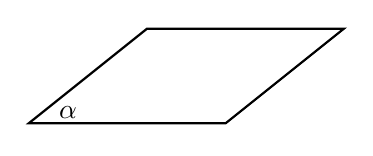
\begin{tikzpicture}
            % Draw parallelogram
            \draw[thick] (0,0) -- (1.5,1.2) -- (4,1.2) -- (2.5,0) -- cycle;
            \node at (0.5,0.13) {$\alpha$};
        \end{tikzpicture}
    }
    \hspace{1cm}
    \subfloat[]{
        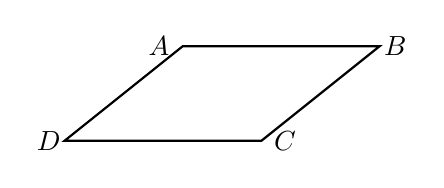
\begin{tikzpicture}
            % Draw parallelogram
            \draw[thick] (0,0) -- (1.5,1.2) -- (4,1.2) -- (2.5,0) -- cycle;
            \node at (1.2,1.2) {$A$};
            \node at (4.2,1.2) {$B$};
            \node at (2.8,0) {$C$};
            \node at (-0.2,0) {$D$};
        \end{tikzpicture}
    }
    \hspace{1cm}
    \subfloat[]{
        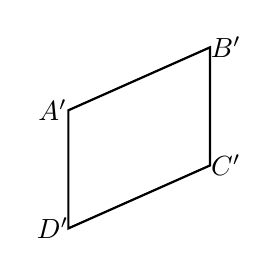
\begin{tikzpicture}
            % Draw parallelogram with different orientation
            \draw[thick] (0,-2) -- (0,-0.5) -- (1.8,0.3) -- (1.8,-1.2) -- cycle;
            \node at (-0.2,-0.5) {$A'$};
            \node at (2,0.3) {$B'$};
            \node at (2,-1.2) {$C'$};
            \node at (-0.2,-2) {$D'$};
        \end{tikzpicture}
    }
    %\caption{Three parallelograms with labels.}
\end{figure}


现在，要在承认平面上的公理的基础上，提出关于空间的公理来刻画平面和其他空间几何体的性质。
公理\ref{欧式公理}的第一条翻译成常见的话就是“两点确定一条直线”，
那么在空间中几个点能确定一个平面呢？
\begin{axiom}\label{基本事实1}
    过不在同一条直线上的三个点，有且仅有一个平面。
\end{axiom}

当然也可以简记为“不共线的三点确定一个平面”。
如右图，\(A,B,C\)作为不共线的三个点，确定了唯一一个平面\(ABC\)。
因此想要确定一个平面，就需要寻找不共线的三个点。

接下来将试图刻画平面的“平”，也就是一个曲面和一个平面应该有什么区别呢？可以考虑使用
直线的“直”来刻画平面的“平”。一个曲面，可以轻松做到直线与之只相交两点，而平面不行。
因此就有了这条公理。
\begin{axiom}
    如果一条直线上两个点在一个平面上，那么这条直线在平面内。
\end{axiom}
用符号刻画就是
\[A\in l,B\in l,A\in \aa,B\in\aa \Rightarrow l\subset \aa\]
注意，这里使用了记号\(l\subset \aa\)，这是因为直线\(l\)和平面\(\aa\)都是点的集合，两个集合的关系自然是“包含”。
换句话说，如果直线在平面内，是指直线上所有的点都在平面上。

在没有这条公理的时候，想判断直线是否在平面内并不容易，这需要检查这条线上所有的点；
但是有这条公理，只看两个点就可以了，
这条公理可以有效判断直线是否在某一平面内。

\begin{exercise}
    尝试说明三角形的三边都在一个平面内。
\end{exercise}


\begin{axiom}
    如果两个不重合的平面有一个公共点，那么它们有且仅有一条过该点的公共直线。
\end{axiom}


接下来使用这三条公理来推理出确定一个平面的其他条件。
\begin{corollary}[确定平面的其他条件]
    \ 

    1. 直线和直线外一点确定一个平面；

    2.两条相交直线确定一个平面。

    3.两条平行直线确定一个平面；
\end{corollary}
\begin{proof}
    1.设直线\(l\)和过直线外一点\(A\)。取\(B,C\in l\)，下面使用反证法说明\(A,B,C\)必然不共线。
    若\(A,B,C\)共线，由两点确定一条直线可知这条直线必然是\(l\)，即\(A\in l\)，与\(A\)是直线外
    一点矛盾。故\(A,B,C\)不共线，确定一个平面\(\aa\)。又\(B\in l,C\in l,B\in\aa,C\in\aa\)，故
    \(l\subset \aa\)，由此一条直线和直线外一点确定一个平面。

    2.记\(l_1\cap l_2=P\)。在\(l_1\)上取一点\(A\)异于\(C\)，在\(l_2\)上取一点\(B\)异于\(C\)。
    下面用反证法来说明\(A,B,P\)不共线。若\(A,B,P\)共线，则应确定唯一一条直线，故\(l_1,l_2\)重合，矛盾！
    由此不共线的\(A,B,P\)确定一个平面\(aa\)。而\(A\in l_1,P\in l_1,A\in \aa,P\in \aa\)，故\(l_1\subset \aa\)，同理
    \(l_2\subset \aa\)，由此两条相交直线确定一个平面。

    3.记\(l_1\pll l_2\)，取\(A,B\in l_1,C\in l_2\)。则\(l_1\)和\(C\)作为直线和直线外
    一点确定一个平面\(\aa\)。下面使用反证法说明\(l_2\subset\aa\)。若\(l_2\not\subset \aa\)，
    则在\(\aa\)内，过\(C\)点存在唯一一条直线\(l_3\pll l_1\)，而\(l_2\cap l_3=C\)，确定一个平面
    \(\bb\)。而\(\aa \text{和}\bb\)交于\(C\)，应仅有一条直线过\(C\)作为两平面的交线，而\(C\in l_2,C\in l_3\)，
    产生矛盾。故\(l_2\subset\aa\)。
    \qed
\end{proof}

\begin{exercise}下面的那些条件可以确定一个平面？
    \begin{enumerate}
        \item 
    \end{enumerate}
\end{exercise}
\clearpage
\subsection{空间中直线与平面的位置关系}

%在空间中一些命题不再成立，比如四个边都相等的四边形是菱形。


\clearpage
\subsection{Hilbert的公理化体系**}
\clearpage

\section{空间几何体}
\subsection{空间几何题的结构与特征}
%简单几何体，组合几何体
\clearpage
\subsection{柱体与锥体}
%拟柱体
\clearpage
\subsection{球}
\clearpage
\subsection{三视图与直观图*}
\clearpage
\chapter{空间中的直线、平面的判定及性质}
\clearpage

\section{直线、平面平行的判定及性质}
\subsection{直线与平面平行}
\clearpage
\subsection{平面与平面平行}
\clearpage

\section{直线、平面垂直的判定及性质}
\subsection{直线与平面垂直}
\clearpage
\subsection{平面与平面垂直}
\clearpage

\section{平行、垂直的综合证明}
\subsection{平形与垂直}
\clearpage
\subsection{空间中的角}
\clearpage
\subsection{空间中的距离}
\clearpage


\chapter{空间向量}


\section{从空间向量到平面向量}
\subsection{空间向量的运算}
%空间版本的基本定理也在这
\clearpage
\subsection{空间直角坐标系}
\clearpage
\subsection{向量的外积}
\clearpage

\section{向量在立体几何中的应用}

\subsection{用向量研究直线与平面}


\clearpage
\subsection{用向量刻画平行和垂直}
\clearpage
\subsection{用向量刻画距离和角度}
\clearpage


\chapter{立体几何的应用}

\section{特殊的空间模型}
\subsection{四面体}
\clearpage
\subsection{截面问题}
\clearpage
\subsection{翻折与反射}
\clearpage


\section{球}
\subsection{球的截面}
\clearpage
\subsection{外接球}
\clearpage
\subsection{内切球}
\clearpage









\chapter{线性代数概览**}%等待大修！
\section{从\texorpdfstring{$\mathbb{R}\text{到}\mathrm{M}_n(\mathbb{F})$}s}
\clearpage
\subsection{线性映射与表示矩阵}
\clearpage
\subsection{线性映射的运算}
\clearpage
\subsection{矩阵的逆与线性方程组}
%不能学完线代连线性方程组都不会解吧！！！
\clearpage

\section{行列式}
\subsection{几种定义}
\clearpage
\subsection{行列式的应用}
\clearpage

\section{线性空间}
\subsection{子空间、基底与维数}
\clearpage
\subsection{矩阵的秩与线性方程组解的结构}
\clearpage

\section{再话内积}
\subsection{内积空间}
Cauthy不等式的统一证明
\subsection{正交矩阵与QR分解}
\clearpage
\subsection{投影与最小二乘}
\clearpage

\section{特征值与特征向量}
\subsection{基础概念}
\clearpage
\subsection{对角化的判据}
\clearpage

\section{二次型}
\subsection{二次型的典范型}
\clearpage
\subsection{实对称矩阵的正交分解}
\clearpage

\chapter{球面上的几何**}

\section{球面上的线和角}
\subsection{从欧式几何看球}
\clearpage
\subsection{球面上的距离和角}
%测地线，大圆为什么好

\clearpage

\section{球面上的几何图形}
\subsection{从两边形到\texorpdfstring{\(n\)}s边形}
%Legendre证明欧拉公式
\clearpage
\subsection{球面三角形的全等}
\clearpage
\subsection{球面上的正余弦定理}
\clearpage






\subsection{非欧几何漫谈}
\clearpage